\documentclass[
	classe=$2^{de}$
]{coursclass}

\usepackage{tikz-repère}
\usetikzlibrary{calc}

\title{Chapitre 6 : Vecteurs dans un repère}
\author{}
\date{}

\begin{document}

\maketitle

\begin{definition}[Base orthonormée]
	\begin{minipage}{0.67\textwidth}
		Soit $O$ un point du plan, et deux vecteurs $\vec{i}$ et $\vec{j}$ dont les directions sont perpendiculaires et dont les normes sont égales à $1$.

		On dit que $(\vec{i},\vec{j})$ est une \textbf{base orthonormée} du plan et que $(O\ ;\ \vec{i},\vec{j})$ est un \textbf{repère orthonormé} du plan.
	\end{minipage}
	\begin{minipage}{0.3\textwidth}
		\begin{center}
			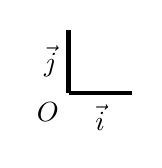
\begin{tikzpicture}[scale=0.8]
				\tikzRepere{-1.5}{1.5}{-1.5}{1.5}[][]
				\node[below left] at (0,0) {$O$};
				\draw[ultra thick,\myArrow] (0,0) -- node[below] {$\vec{i}$} ++(1,0);
				\draw[ultra thick,\myArrow] (0,0) -- node[left] {$\vec{j}$} ++(0,1);
			\end{tikzpicture}
		\end{center}
	\end{minipage}
\end{definition}

\begin{propriete}[Coordonnées d'un vecteur]
	\begin{minipage}{0.65\textwidth}
		Si $(\vec{i},\vec{j})$ est une base orthonormée du plan et $u$ est un vecteur, il existe un unique couple de réels $(x\ ;\ y)$ tel que :

		$$\vec{u} = x\vec{i} + y\vec{j}$$

		On dit que le vecteur $\vec{u}$ a pour \textbf{coordonnées} $\begin{pmatrix} x \\ y \end{pmatrix}$ dans la base $(\vec{i},\vec{j})$.
	\end{minipage}
	\begin{minipage}{0.3\textwidth}
		\begin{center}
			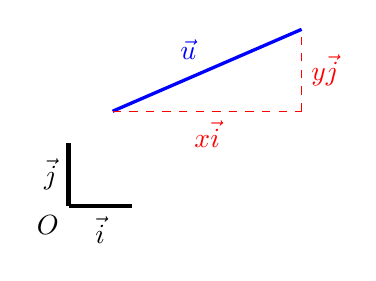
\begin{tikzpicture}[scale=0.8]
				\coordinate (VecX) at (3,0);
				\coordinate (VecY) at (0,1.3);
				\coordinate (StartVec) at (0.7,1.5);
				\tikzRepere{-0.5}{4.5}{-0.5}{3.5}[][]
				\node[below left] at (0,0) {$O$};
				\draw[ultra thick,\myArrow] (0,0) -- node[below] {$\vec{i}$} ++(1,0);
				\draw[ultra thick,\myArrow] (0,0) -- node[left] {$\vec{j}$} ++(0,1);
				\draw[very thick,blue,\myArrow] (StartVec) -- node[above left] {$\vec{u}$} ++($(VecX) + (VecY)$);
				\draw[dashed,red,\myArrow] (StartVec) -- node[below] {$x\vec{i}$} ++(VecX);
				\draw[dashed,red,\myArrow] (StartVec) ++(VecX) -- node[right] {$y\vec{j}$} ++(VecY);
			\end{tikzpicture}
		\end{center}
	\end{minipage}
\end{propriete}

\begin{remarque}
	\begin{itemize}
		\item Cela revient à décomposer le vecteur $\vec{u}$ en sa composante horizontale et verticale.
		\item Deux vecteurs sont égaux si et seulement si leurs coordonnées sont égales.
		\item On écrit les coordonnées d'un \uline{point} à l'horizontale, et celles d'un \uline{vecteur} à la verticale :

		      \begin{center}
			      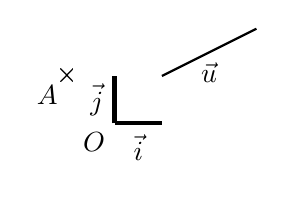
\begin{tikzpicture}[scale=0.6]
				      \tikzRepere{-1.5}{3.5}{-0.5}{2.5}[][]
				      \node[below left] at (0,0) {$O$};
				      \draw[ultra thick,\myArrow] (0,0) -- node[below] {$\vec{i}$} ++(1,0);
				      \draw[ultra thick,\myArrow] (0,0) -- node[left] {$\vec{j}$} ++(0,1);
				      \draw[thick,\myArrow] (1,1) -- node[below] {$\vec{u}$} ++(2,1);

				      \coordinate (A) at (-1,1);
				      \node at (A) {×};
				      \node[below left] at (A) {$A$};
			      \end{tikzpicture}
		      \end{center}
		      \begin{align*}
			      A & (-1 ; 1) & \vec{u} & \begin{pmatrix}2 \\ 1\end{pmatrix}
		      \end{align*}
	\end{itemize}
\end{remarque}

\begin{exemple}
	\begin{center}
		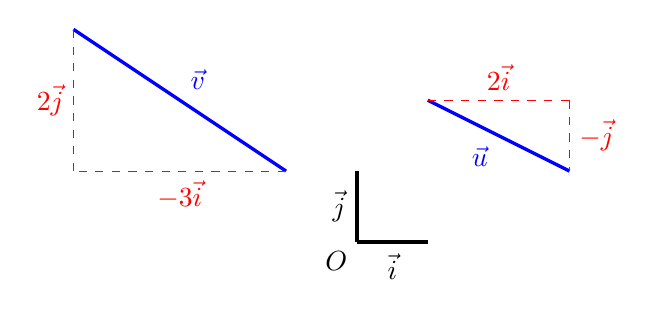
\begin{tikzpicture}[scale=0.9]
			\coordinate (StartU) at (1,2);
			\coordinate (StartV) at (-1,1);
			\coordinate (Ux) at (2,0);
			\coordinate (Uy) at (0,-1);
			\coordinate (Vx) at (-3,0);
			\coordinate (Vy) at (0,2);

			\tikzRepere{-4.5}{3.5}{-0.5}{3.5}[][]
			\node[below left] at (0,0) {$O$};
			\draw[ultra thick,\myArrow] (0,0) -- node[below] {$\vec{i}$} ++(1,0);
			\draw[ultra thick,\myArrow] (0,0) -- node[left] {$\vec{j}$} ++(0,1);

			\draw[very thick,blue,\myArrow] (StartU) -- node[below left] {$\vec{u}$} ++($(Ux) + (Uy)$);
			\draw[dashed,red,\myArrow] (StartU) -- node[above] {$2\vec{i}$} ++(Ux);
			\draw[dashed,red,\myArrow] ($(StartU) + (Ux)$) -- node[right] {$-\vec{j}$} ++(Uy);

			\draw[very thick,blue,\myArrow] (StartV) -- node[above right] {$\vec{v}$} ++($(Vx) + (Vy)$);
			\draw[dashed,red,\myArrow] (StartV) -- node[below] {$-3\vec{i}$} ++(Vx);
			\draw[dashed,red,\myArrow] ($(StartV) + (Vx)$) -- node[left] {$2\vec{j}$} ++(Vy);
		\end{tikzpicture}
	\end{center} \medskip

	Dans le repère ci-dessus, on a
	\begin{itemize}
		\item $\vec{u} = 2\vec{i} - \vec{j}$, donc $\vec{u}\begin{pmatrix} 2 \\ -1 \end{pmatrix}$ dans la base $(\vec{i},\vec{j})$.
		\item $\vec{v} = -3\vec{i} + 2\vec{j}$, donc $\vec{v}\begin{pmatrix} -3 \\ 2 \end{pmatrix}$ dans la base $(\vec{i},\vec{j})$.
	\end{itemize}
\end{exemple}

\begin{propriete}[Coordonnées d'un vecteur à partir de points]
	Soient $A(x_A\ ;\ y_A)$ et $B(x_B\ ;\ y_B)$ deux points du plan.

	Alors le vecteur $\vec{AB}$ a pour coordonnées
	$$ \begin{pmatrix}
			x_B - x_A \\
			y_B - y_A
		\end{pmatrix} $$
\end{propriete}

\begin{exemple}
	\begin{center}
		\begin{tikzpicture}[scale=0.9]
			\coordinate (A) at (1,3);
			\coordinate (B) at (5,0);

			\tikzRepere{-0.5}{5.5}{-0.5}{3.5}[][]
			\node[below left] at (0,0) {$O$};
			\draw[ultra thick,\myArrow] (0,0) -- node[below] {$\vec{i}$} ++(1,0);
			\draw[ultra thick,\myArrow] (0,0) -- node[left] {$\vec{j}$} ++(0,1);

			\node at (A) {×};
			\node[below] at (A) {$A$};
			\node at (B) {×};
			\node[below] at (B) {$B$};
			\draw[thick,red,\myArrow] (A) -- node[above] {$\vec{AB}$} (B);
		\end{tikzpicture}
	\end{center} \medskip

	Dans le repère ci-dessus, on a les points $A(1\ ;\ 3)$ et $B(5\ ;\ 0)$.

	Donc le vecteur $\vec{AB}$ a pour coordonnées $\begin{pmatrix} 5 - 1 \\ 0 - 3 \end{pmatrix} = \begin{pmatrix} 4 \\ -3 \end{pmatrix}$.
\end{exemple}

\begin{propriete}[Norme d'un vecteur]
	Si un vecteur $\vec{u}$ a pour coordonnées $\begin{pmatrix} x \\ y \end{pmatrix}$, sa norme est égale à $‖\vec{u}‖ = \sqrt{x² + y²}$.
\end{propriete}

\begin{exemple}
	\begin{minipage}{0.65\textwidth}
		Soit $\vec{u}\begin{pmatrix} 3 \\ -2 \end{pmatrix}$.

		Alors $‖\vec{u}‖ = \sqrt{3² + (-2)²} = \sqrt{9 + 4} = \sqrt{13}$. \bigskip

		Remarquons que cela revient à calculer la distance entre les deux extrémités du vecteur.
	\end{minipage}
	\begin{minipage}{0.3\textwidth}
		\begin{center}
			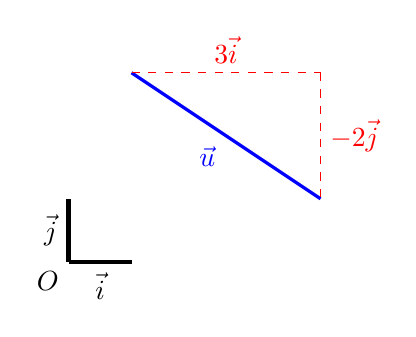
\begin{tikzpicture}[scale=0.8]
				\tikzRepere{-0.5}{5.5}{-0.5}{3.5}[][]
				\node[below left] at (0,0) {$O$};
				\draw[ultra thick,\myArrow] (0,0) -- node[below] {$\vec{i}$} ++(1,0);
				\draw[ultra thick,\myArrow] (0,0) -- node[left] {$\vec{j}$} ++(0,1);

				\draw[very thick,blue,\myArrow] (1,3) -- node[below left] {$\vec{u}$} (4,1);
				\draw[dashed,red,\myArrow] (1,3) -- node[above] {$3\vec{i}$} (4,3);
				\draw[dashed,red,\myArrow] (4,3) -- node[right] {$-2\vec{j}$} (4,1);
			\end{tikzpicture}
		\end{center}
	\end{minipage}
\end{exemple}

\begin{propriete}[Somme de vecteurs]
	Si on a deux vecteurs $\vec{u}\begin{pmatrix} x \\ y \end{pmatrix}$ et $\vec{v}\begin{pmatrix} x' \\ y' \end{pmatrix}$, alors $\vec{u} + \vec{v}$ a pour coordonnées $\begin{pmatrix} x + x' \\ y + y' \end{pmatrix}$.
\end{propriete}

\begin{exemple}
	Soit $\vec{u}\begin{pmatrix} 3 \\ -5 \end{pmatrix}$ et $\vec{v}\begin{pmatrix} -1 \\ 4 \end{pmatrix}$. Alors $\vec{u} + \vec{v}$ a pour coordonnées $\begin{pmatrix} 3 + (-1) \\ -5 + 4 \end{pmatrix} = \begin{pmatrix} 2 \\ -1 \end{pmatrix}$.
\end{exemple}

\begin{propriete}[Produit d'un vecteur par un réel]
	Si un vecteur $\vec{u}$ a pour coordonnées $\begin{pmatrix} x \\ y \end{pmatrix}$ et $k$ est un nombre réel, le vecteur $k\vec{u}$ a pour coordonnées $\begin{pmatrix} kx \\ ky \end{pmatrix}$.
\end{propriete}

\begin{exemple}
	Soit $\vec{u}\begin{pmatrix} -2 \\ 5 \end{pmatrix}$. Alors le vecteur $-3\vec{u}$ a pour coordonnées $\begin{pmatrix} -3 × (-2) \\ -3 × 5 \end{pmatrix} = \begin{pmatrix} 6 \\ -15 \end{pmatrix}$.
\end{exemple}

\begin{definition}[Colinéarité]
	Si deux vecteurs ont la même direction, on dit qu'ils sont \textbf{colinéaires}.
\end{definition}

\begin{propriete}[Colinéarité]
	Si $\vec{u}\begin{pmatrix} x \\ y \end{pmatrix}$ et $\vec{v}\begin{pmatrix} x' \\ y' \end{pmatrix}$, alors $\vec{u}$ et $\vec{v}$ sont colinéaires si, de manière équivalente, on a : \medskip

	\begin{minipage}{0.7\textwidth}
		\begin{itemize}
			\item $\vec{u} = k\vec{v}$, avec $k$ un nombre réel ;
			\item Les coordonnées de $\vec{u}$ et $\vec{v}$ sont proportionnelles ;
			\item $x × y' = x' × y$
		\end{itemize}
	\end{minipage}
	\begin{minipage}{0.25\textwidth}
		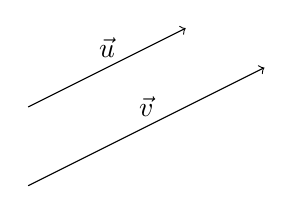
\begin{tikzpicture}
			\draw[->] (0,1) -- node[above] {$\vec{u}$} ++(2,1);
			\draw[->] (0,0) -- node[above] {$\vec{v}$} ++(3,1.5);
		\end{tikzpicture}
	\end{minipage}
\end{propriete}

\begin{exemple}
	Les vecteurs $\begin{pmatrix}6 \\ 15\end{pmatrix}$ et $\begin{pmatrix}4 \\ 10\end{pmatrix}$ sont colinéaires, car $6 × 10 = 4 × 15 ( = 60)$.
\end{exemple}

\begin{propriete}[Milieu d'un segment]
	Si on a deux points $A(x_A ; y_A)$ et $B(x_B ; y_B)$, le milieu $M$ du segment $[AB]$ a pour coordonnées $M\left(\dfrac{x_A + x_B}{2}; \dfrac{y_A + y_B}{2}\right)$.
\end{propriete}

\begin{exemple}
	\begin{center}
		\begin{tikzpicture}[scale=0.7]
			\tikzRepere{-0.5}{8.5}{-0.5}{5.5}[][]
			\node[below left] at (0,0) {$O$};
			\draw[thick,\myArrow] (0,0) -- node[below] {$\vec{i}$} (1,0);
			\draw[thick,\myArrow] (0,0) -- node[left] {$\vec{j}$} (0,1);

			\coordinate (A) at (2,0);
			\coordinate (B) at (8,4);
			\coordinate (M) at ($(A)!0.5!(B)$);

			\foreach \p in {A,B,M} {
				\node at (\p) {×};
				\node[above left] at (\p) {$\p$};
			}
			\draw (A) -- (B);
		\end{tikzpicture}
	\end{center}
	Sur la figure ci-dessus, on a $A(2;0)$ et $B(8;4)$. Ainsi le milieu de $[AB]$ a pour coordonnées 
	
	$M\left(\dfrac{2+8}{2} ; \dfrac{0+4}{2}\right) = (5 ; 2)$.
\end{exemple}

\end{document}